\documentclass[25pt, a0paper, portrait, margin=0mm, innermargin=20mm,
blockverticalspace=2mm, colspace=20mm, subcolspace=0mm]{tikzposter} %Default values for poster format options.

\usepackage[utf8]{inputenc}
\usepackage[scaled]{helvet}
\renewcommand\familydefault{\sfdefault} 
\usepackage[T1]{fontenc}
\usepackage{wrapfig}
\usepackage{setspace}
\usepackage{multicol}
\setlength{\columnsep}{1.5cm}
\usepackage{xspace}
\usepackage{tikz}
\tikzposterlatexaffectionproofoff
\usetheme{Default}

\definecolor{text}{HTML}{e0e4f7}
\definecolor{background}{HTML}{111116}
\definecolor{boxes}{HTML}{2a2a32}
\definecolor{unired}{HTML}{a51e37}

\colorlet{blocktitlefgcolor}{text}
\colorlet{backgroundcolor}{background}
\colorlet{blocktitlebgcolor}{background}
\colorlet{blockbodyfgcolor}{text}
\colorlet{innerblocktitlebgcolor}{background}
\colorlet{innerblocktitlefgcolor}{text}
\colorlet{notefrcolor}{text}
\colorlet{notefgcolor}{background}
\colorlet{notebgcolor}{background}


% Title setup
\settitle{
% Rearrange the order of the minipages to e.g. center the title between the logos
\begin{minipage}[c]{0.8\paperwidth}
%    \centering
    \vspace{2.5cm}\hspace{1.5cm}
    \color{text}{\Huge{\textbf{\@title}} \par}
    \vspace*{2em}\hspace{1.5cm}
    \color{text}{\LARGE \@author \par}
    \vspace*{2em}\hspace{1.5cm}
    \color{text}{\Large \@institute}
    \vspace{2.5cm}
\end{minipage}
\begin{minipage}[c]{0.2\paperwidth}
    \centering
    % \vspace{1cm}
    \hspace{-7cm}
    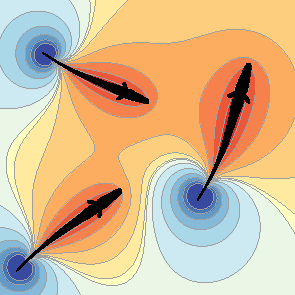
\includegraphics[width=0.7\linewidth]{figs/efishlogo.pdf}
\end{minipage}}
% \begin{minipage}[c]{0.2\paperwidth}
%     \vspace{1cm}\hspace{1cm}
%     \centering
%     \includegraphics[width=\linewidth]{example-image-a}
% \end{minipage}}

% define title style with background box (currently white)
\definetitlestyle{sampletitle}{
    width=841mm,
    roundedcorners=0,
    linewidth=0pt,
    innersep=15pt,
    titletotopverticalspace=0mm,
    titletoblockverticalspace=5pt
}{
    \begin{scope}[line width=\titlelinewidth,
        rounded corners=\titleroundedcorners]
    \draw[fill=text, color=boxes]
    (\titleposleft,\titleposbottom)
    rectangle
    (\titleposright,\titlepostop);
    \end{scope}
}

% define coustom block style for visible blocks
\defineblockstyle{GrayBlock}{
    titlewidthscale=1,
    bodywidthscale=1,
    % titlecenter,
    titleleft,
    titleoffsetx=0pt,
    titleoffsety=-30pt,
    bodyoffsetx=0pt,
    bodyoffsety=-40pt,
    bodyverticalshift=0mm,
    roundedcorners=25,
    linewidth=1pt,
    titleinnersep=20pt,
    bodyinnersep=38pt
}{
    \draw[rounded corners=\blockroundedcorners, inner sep=\blockbodyinnersep,
          line width=\blocklinewidth, color=background,
          top color=boxes, bottom color=boxes,
          ]
      (blockbody.south west) rectangle (blockbody.north east); %
    \ifBlockHasTitle%
        \draw[rounded corners=\blockroundedcorners, inner sep=\blocktitleinnersep,
          top color=background, bottom color=background,
          line width=2, color=background, %fill=blocktitlebgcolor
          ]
      (blocktitle.south west) rectangle (blocktitle.north east); %
    \fi%
}
\newcommand\myblock[3][GrayBlock]{\useblockstyle{#1}\block{#2}{#3}\useblockstyle{Default}}

% Define blockstyle for tranparent block
\defineblockstyle{TranspBlock}{
    titlewidthscale=0.99,
    bodywidthscale=0.99,
    titleleft,
    titleoffsetx=15pt,
    titleoffsety=-40pt,
    bodyoffsetx=0pt,
    bodyoffsety=-40pt,
    bodyverticalshift=0mm,
    roundedcorners=25,
    linewidth=1pt,
    titleinnersep=20pt,
    bodyinnersep=38pt
}{
    \draw[rounded corners=\blockroundedcorners, inner sep=\blockbodyinnersep,
          line width=\blocklinewidth, color=background,
          top color=background, bottom color=background,
          ]
      (blockbody.south west) rectangle (blockbody.north east); %
    \ifBlockHasTitle%
        \draw[rounded corners=\blockroundedcorners, inner sep=\blocktitleinnersep,
          top color=background, bottom color=background,
          line width=2, color=background, %fill=blocktitlebgcolor
          ]
      (blocktitle.south west) rectangle (blocktitle.north east); %
    \fi%
}
\renewcommand\myblock[3][TranspBlock]{\useblockstyle{#1}\block{#2}{#3}\useblockstyle{Default}}


\begin{document}
 
\renewcommand{\baselinestretch}{1} 
\title{\parbox{1500pt}{Complex frequency modulations in freely interacting electric fish, \textit{Apteronotus leptorhynchus}, recorded in their natural habitat}}
\author{Patrick Weygoldt, Till Raab, Jan Benda}
\institute{Neuroethology Lab, Department of Neurobiology, University of Tuebingen}
\usetitlestyle[]{sampletitle}
\maketitle
\renewcommand{\baselinestretch}{1.4} 

\begin{columns}
\column{0.3333}
\myblock[MyBlock]{Introduction}{
    Weakly electric fish use their electric organ discharge (EOD) for navigation, foraging and \textbf{communication}. Signals associated with communication (chirps and rises) are extensively studied and can be identified by their stereotyped EOD frequency (EOD$f$) modulations. But signals that are not as stereotyped receive little attention. For a \textbf{natural population} of \textit{A. leptorhynchus}, recorded using an array of 64 electrodes, we find \textbf{synchronous} EOD$f$ modulations lasting many minutes. We designed a simple algorithm to detect synchronous modulations in two animals and analyzed their movements during frequency interactions.
    \vspace{0.6cm}
    \begin{tikzfigure}[]
        \label{griddrawing}
        \includegraphics[width=\linewidth]{figs/dsc_2193_02.jpg}
    \end{tikzfigure} 
}

\myblock[MyBlock]{Event detection}{
    Detection of synchrony:
    \begin{enumerate}
        \setlength\itemsep{0.5em}
        \item Extract pairwise EOD$f$ tracks (\textbf{A}).
        \item Bandpass-filter on two time scales (\textbf{B}).
        \item \textbf{Sliding-window cross-covariances} of filtered track-pairs, extract maxima across all lags (black line, \textbf{C}).
        \item Detect peaks in covariances. Simultaneously co-occurring covariance peaks are "events" (\textbf{D}).
        \item Manual validation of detected synchronous modulations using a minimalist GUI.
    \end{enumerate}
    Detection of physical interactions using proximity, velocity and relative angle of heading trajectories between fish.
    \vspace{0.85cm}
    \begin{tikzfigure}[]
        \label{detector}
        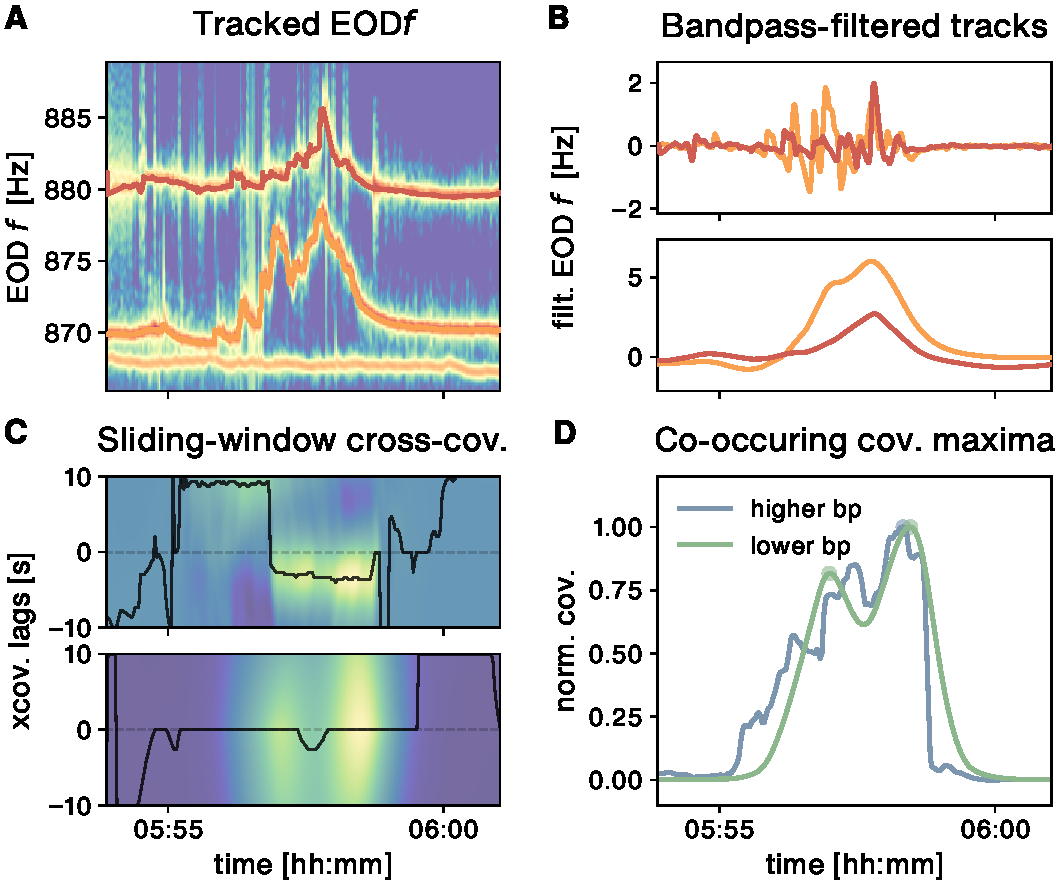
\includegraphics[width=\linewidth]{figs/CovDetector_backend_ids_26788_26789_index_0.pdf}
    \end{tikzfigure} 
    \vspace{0cm}
}

\column{0.6666}
\myblock[MyBlock]{Detected modulations}{
    
    We found phases of synchrony up to 50 Hz in $\Delta$EOD$f$ that lasted for over 10 minutes. 
    Synchronous modulations ranged from clearly distinguishable and steep rises to smooth modulations with low EOD$f$ increases.

    \vspace{0.4cm}

    \begin{tikzfigure}[]
        \label{modulations}
        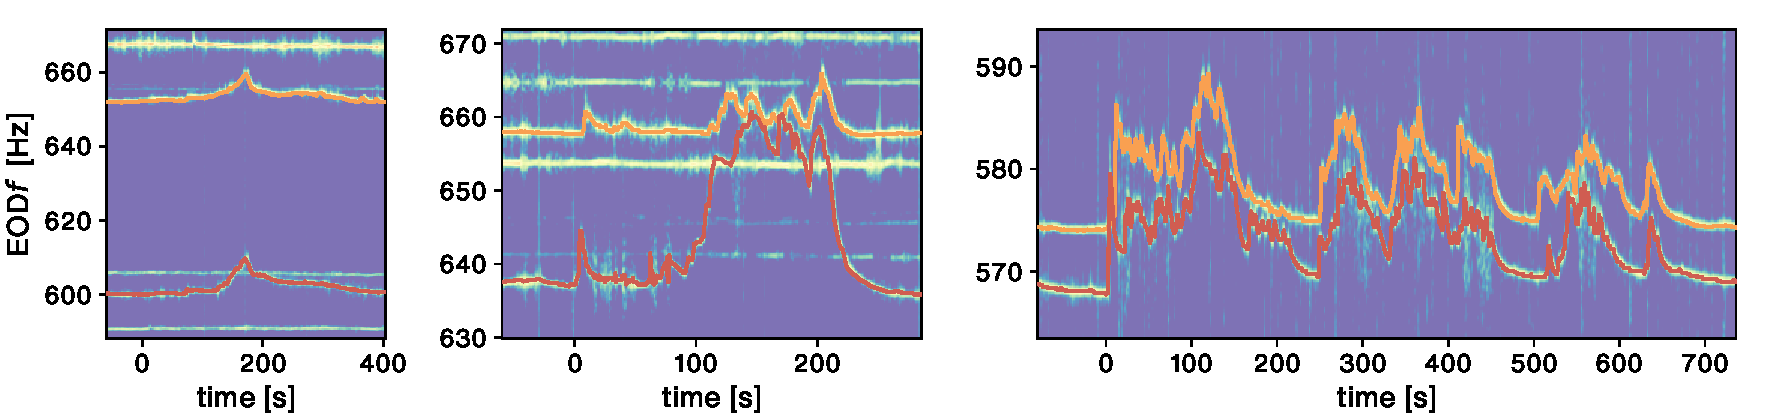
\includegraphics[width=\linewidth]{figs/selected_modulations.pdf}
    \end{tikzfigure}
    \vspace{0.2cm}
    \begin{tikzfigure}[]
        \label{eventpos}
        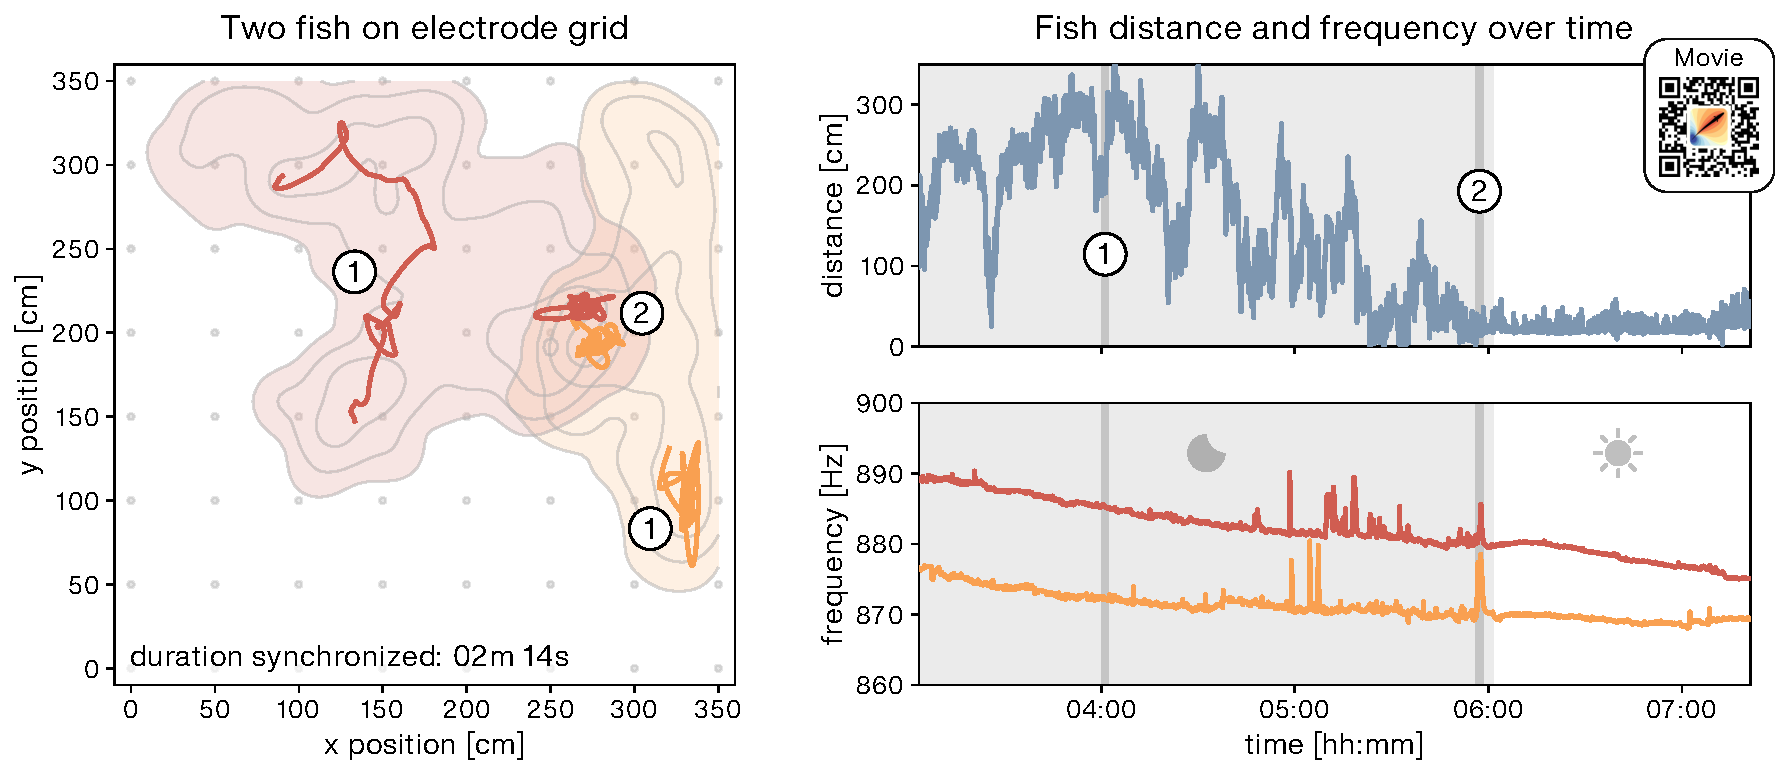
\includegraphics[width=\linewidth]{figs/eventposition_2.pdf}
    \end{tikzfigure} 

    \noindent
}

\myblock[MyBlock]{Interactions at modulations}{
    \vspace{-1.2cm}
    \begin{tikzfigure}[]
        \label{results}
        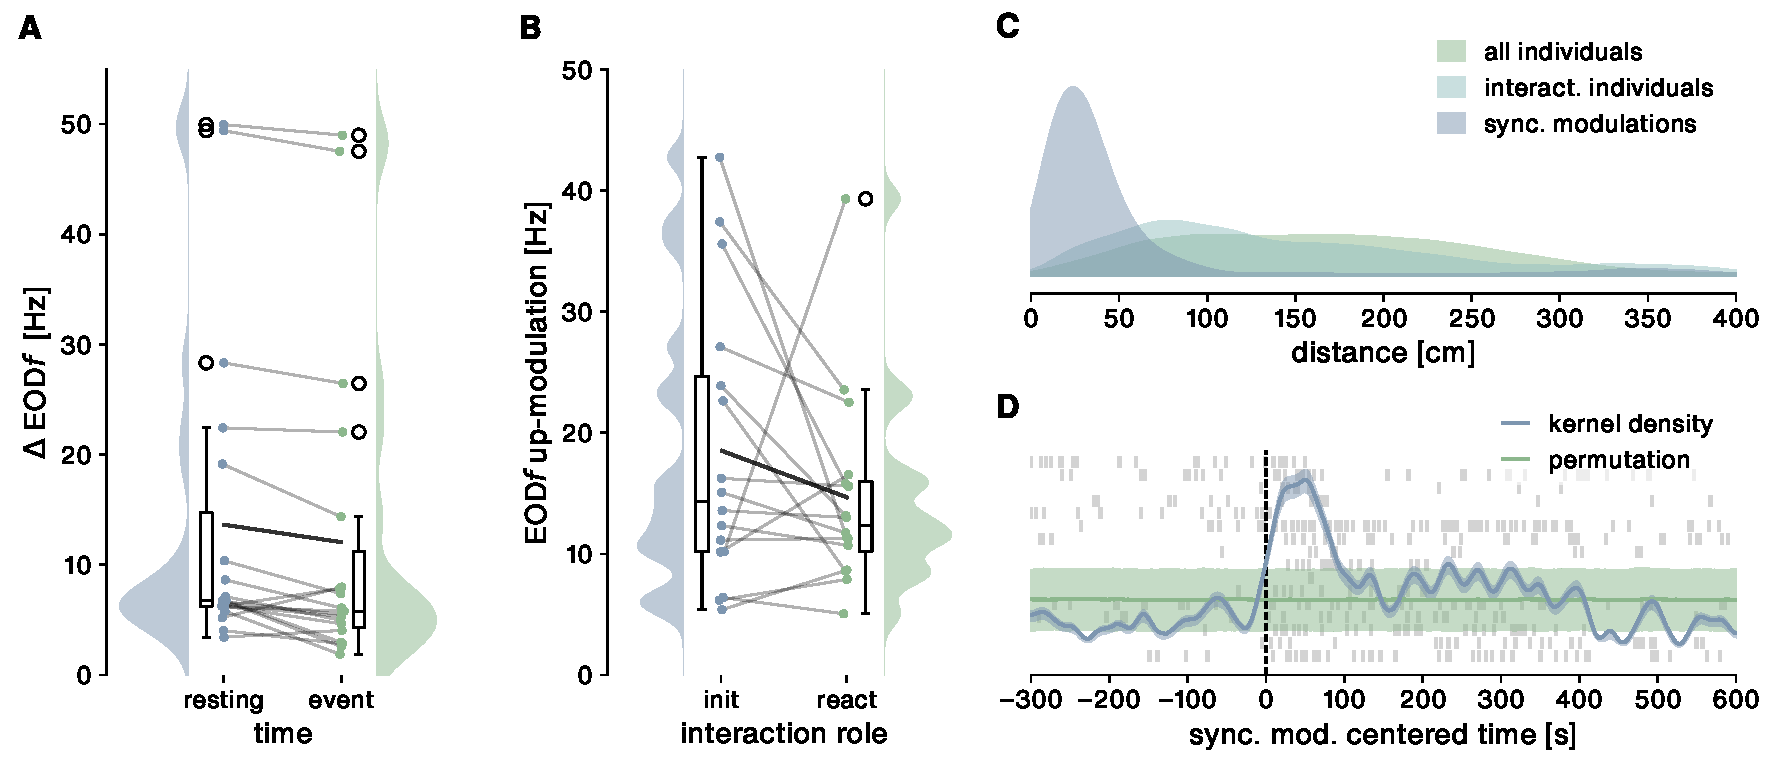
\includegraphics[width=\linewidth]{figs/eventstats.pdf}
    \end{tikzfigure}

    \begin{multicols}{2}
        \begin{itemize}
            \setlength\itemsep{0.5em}
            \item $\Delta$EOD$f$ does not appear to decrease during synchronous modulations (\textbf{A}).
            \item Individuals that rise their EOD$f$ first appear to rise their frequency higher compared to reactors (\textbf{B}).
            \vfill
            \null
            \columnbreak
            \item Synchronized fish keep distances below 1 m (\textbf{C}) but distances over 3 m also occur (see \textbf{movie}).
            \item Spatial interactions increase \textbf{after} the start of a synchronous modulation (\textbf{D}).
        \end{itemize}
    \end{multicols}
    \vspace{-1cm}
}

\myblock[MyBlock]{Conclusion}{
    \begin{itemize}
        \setlength\itemsep{0.5em}
        \item Our analysis is the first to indicate that \textit{A. leptorhynchus} uses long, diffuse and synchronized EOD$f$ signals to communicate in addition to chirps and rises.
        \item The recorded fish do not exhibit jamming avoidance behavior while close during synchronous modulations.
        \item Synchronous signals \textbf{initiate} spatio-temporal interactions.
    \end{itemize}
    \vspace{0.2cm}
    }
\end{columns}

\node [above right, text=white, outer sep=45pt,minimum width=\paperwidth, align=center, draw, fill=unired, color=unired] at (-43.6,-61) { \textcolor{white}{\normalsize Contact: patrick.weygoldt@student.uni-tuebingen.de}};

\end{document}